% This section should reintroduce the full data flow diagram from the architectural specification, and discuss at a high level the purpose of each layer. You do not need to include a subsection for each layer, a 1 - 2 paragraph recap is sufficient.

\begin{figure}[h!]
	\centering
 	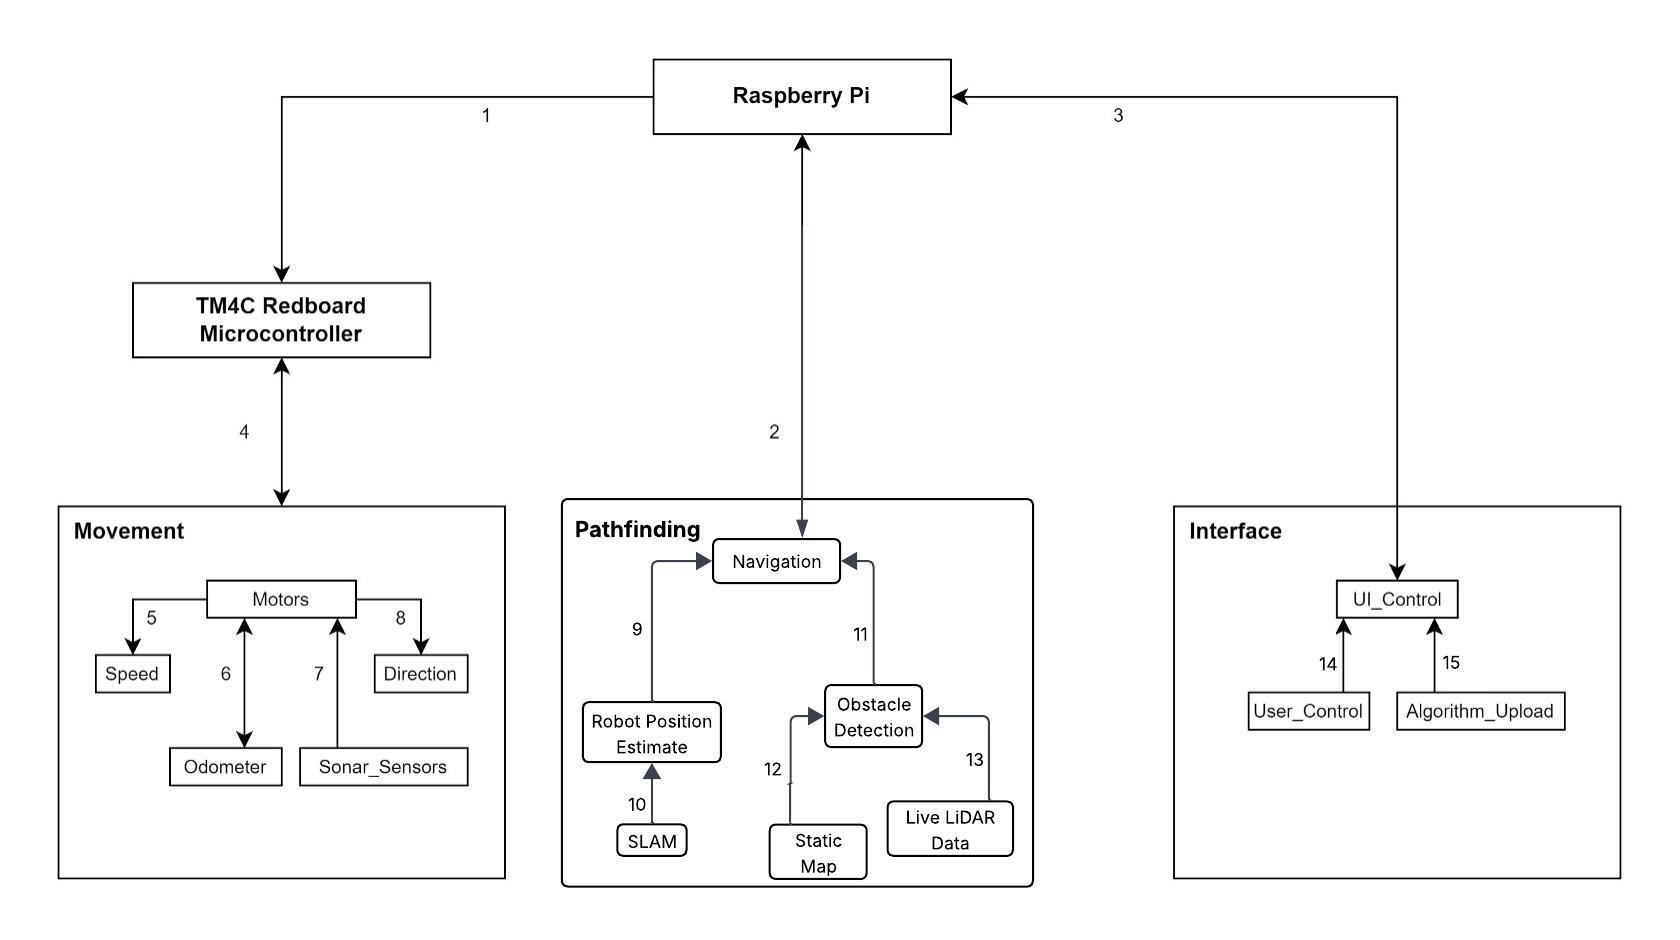
\includegraphics[width=1\textwidth]{images/data_flow_2nd.jpeg}
 \caption{Data Flow Diagram}
\end{figure}

The architecture of the RoamBot system is structured into three distinct layers: Movement, Path Finding, and Interface, each serving a critical role in the rover's functionality. The Movement Layer is responsible for controlling the rover's motion, including speed, direction, and crash prevention. It utilizes UART to control speed and direction and GPIO for safety features like stopping when obstacles are detected. The Path Finding Layer enables autonomous navigation through LIDAR-based mapping and obstacle detection, using GPIO communication with a TM4C microcontroller to control and guide the movement. Lastly, the Interface Layer acts as the bridge between the user and the system, handling user command interactions, including direct control of the rover and algorithm uploads.

These layers work together to ensure efficient and autonomous operation of the RoamBot. The Movement Layer executes physical actions based on inputs from the Path Finding Layer, which interprets environmental data to determine safe navigation paths. The Interface Layer facilitates user interaction, allowing for both manual and automated control. This structured approach ensures modularity, making each layer functionally independent while maintaining well-defined communication interfaces for seamless operation.
